\documentclass{standalone}
\usepackage{tikz}
\usetikzlibrary{shapes,arrows.meta}
\begin{document}
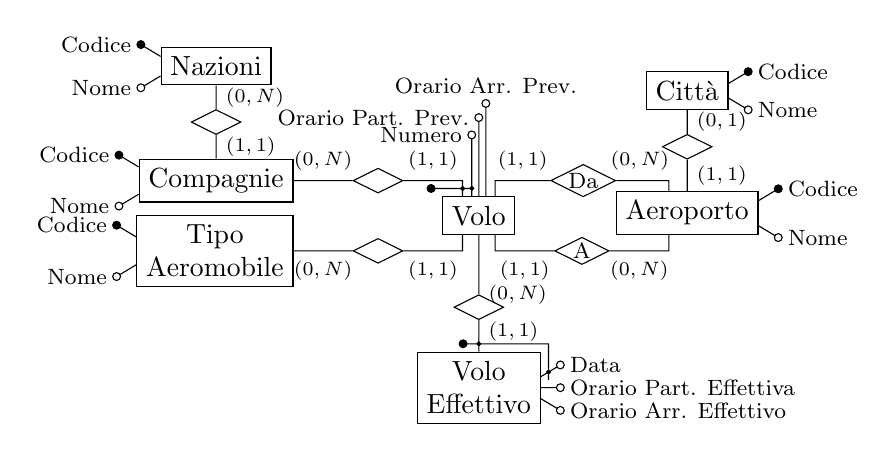
\begin{tikzpicture}
    \draw

    %%* Attributi:
    %%  node[draw, circle, inner sep=1pt, fill=black]{}node[right]{\footnotesize A}
    %%  node[draw, circle, inner sep=0.5pt, fill=black](a){}
    %%? Distanza orizzontale: E -(0.25,0.x)- A
    %%? Distanza verticale: E -(0,x * 0.22)- A

    %%* Cardinalità:
    %%  node[below right]{\scriptsize $(0,N)$}
    %%  node[above right]{\scriptsize $(0,N)$}
    %%  node[midway, above]{\scriptsize $(0,N)$}

    %%* Relazione:
    %%  node[draw, diamond, shape aspect=2, inner sep=3pt, anchor=90](r1){}
    %%  node[draw, diamond, shape aspect=2, inner sep=0.2pt, anchor=180](r2){R2}

    %%* Entità:
    %%  node[draw, rectangle, anchor=90](e1){}
    %%? Distanza verticale: E -(0.3)- R -(0.3) E
    %%? Distanza orizzontale: E -(0.75)- R -(0.75)- E

    %%* Nazioni
    (0,0)node[draw, rectangle, anchor=90](naz){Nazioni}
    (naz.170)--++(-0.25,.15)node[draw, circle, inner sep=1pt, fill=black]{}node[left]{\footnotesize Codice}
    (naz.190)--++(-.25,-.15)node[draw, circle, inner sep=1pt, fill=white]{}node[left]{\footnotesize Nome}
    
    %%* Compagnie
    (naz.270)--++(0,-0.3)node[midway, right]{\scriptsize $(0,N)$}node[draw, diamond, shape aspect=2, inner sep=3pt, anchor=90](r1){}
    (r1.270)--++(0,-0.3)node[draw, rectangle, anchor=90](cmp){Compagnie}node[midway, right]{\scriptsize $(1,1)$}
    (cmp.170)--++(-0.25,.15)node[draw, circle, inner sep=1pt, fill=black]{}node[left]{\footnotesize Codice}
    (cmp.190)--++(-.25,-.15)node[draw, circle, inner sep=1pt, fill=white]{}node[left]{\footnotesize Nome}

    %%* Volo
    (cmp.0)--++(0.75,0)node[midway, above]{\scriptsize $(0,N)$}node[draw, diamond, shape aspect=2, inner sep=3pt, anchor=180](r2){}
    (r2.0)--++(0.75,0)node[midway, above]{\scriptsize $(1,1)$}--++(0,-0.1)node[draw, circle, inner sep=0.5pt, fill=black](b){}--++(0,-0.1)node[draw, rectangle, anchor=130](vol){Volo}
    (vol.110)--++(0,0.1)node[draw, circle, inner sep=0.5pt, fill=black](a){}--++(0,0.68)node[draw, circle, inner sep=1pt, fill=white]{}node[left]{\footnotesize Numero}
    (vol.90)--++(0,1)node[draw, circle, inner sep=1pt, fill=white]{}node[left]{\footnotesize Orario Part. Prev.}
    (vol.70)--++(0,1.18)node[draw, circle, inner sep=1pt, fill=white]{}node[above]{\footnotesize Orario Arr. Prev.}

    (b)++(-0.4,0)node[draw, circle, inner sep=1pt, fill=black]{}--(a)--++(0,0.1)

    %%%* Aeroporto  
    %%* A
    (vol.310)--++(0,-0.2)--++(0.75,0)node[midway, below]{\scriptsize $(1,1)$}node[draw, diamond, shape aspect=2, inner sep=0.4pt, anchor=180](r2){\footnotesize A}
    (r2.0)   --++(0.75,0)node[midway, below]{\scriptsize $(0,N)$}--++(0,0.2)node[draw, rectangle, anchor=230](aep){Aeroporto}
    %%* Da
    (vol.50)--++(0,0.2) --++(0.7,0)node[midway, above]{\scriptsize $(1,1)$}node[draw, diamond, shape aspect=2, inner sep=0.3pt, anchor=180](r2){\footnotesize Da}
    (r2.0)--++(0.6,0)node[midway, above]{\scriptsize $(0,N)$}-|(aep.130)
    
    (aep.10)--++(0.25,.15)node[draw, circle, inner sep=1pt, fill=black]{}node[right]{\footnotesize Codice}
    (aep.350)--++(.25,-.15)node[draw, circle, inner sep=1pt, fill=white]{}node[right]{\footnotesize Nome}


    %%* Città
    (aep.90)--++(0,0.4)node[midway, right]{\scriptsize $(1,1)$}node[draw, diamond, shape aspect=2, inner sep=3pt, anchor=270](r1){}
    (r1.90)--++(0,0.3)node[midway, right]{\scriptsize $(0,1)$}node[draw, rectangle, anchor=270](cit){Città}
    (cit.10)--++(0.25,.15)node[draw, circle, inner sep=1pt, fill=black]{}node[right]{\footnotesize Codice}
    (cit.350)--++(.25,-.15)node[draw, circle, inner sep=1pt, fill=white]{}node[right]{\footnotesize Nome}
    
    %%* Tipo Aeromobile
    (vol.230)--++(0,-0.2)--++(-0.75,0)node[midway, below]{\scriptsize $(1,1)$}node[draw, diamond, shape aspect=2, inner sep=3pt, anchor=0](r1){}
    (r1.180) --++(-0.75,0)node[midway, below]{\scriptsize $(0,N)$}node[draw, rectangle, anchor=0, align=center](tip){Tipo\\Aeromobile}
    (tip.170)--++(-0.25,.15)node[draw, circle, inner sep=1pt, fill=black]{}node[left]{\footnotesize Codice}
    (tip.190)--++(-.25,-.15)node[draw, circle, inner sep=1pt, fill=white]{}node[left]{\footnotesize Nome}
    
    %%* Volo Effettivo
    (vol.270)--++(0,-0.75)node[right]{\scriptsize $(0,N)$}node[draw, diamond, shape aspect=2, inner sep=3pt, anchor=90](r1){}
    (r1.270)--++(0,-0.3)node[midway, right]{\scriptsize $(1,1)$}node[draw, circle, inner sep=0.5pt, fill=black](a){}--++(0,-0.1)node[draw, rectangle, anchor=90, align=center](vole){Volo\\Effettivo}
    (vole.10)--++(0.1,0.06)node[draw, circle, inner sep=0.5pt, fill=black](b){}--++(0.15,0.09)node[draw, circle, inner sep=1pt, fill=white]{}node[right]{\footnotesize Data}
    (vole.0)--++(.25,0)node[draw, circle, inner sep=1pt, fill=white]{}node[right]{\footnotesize Orario Part. Effettiva}
    (vole.350)--++(.25,-.15)node[draw, circle, inner sep=1pt, fill=white]{}node[right]{\footnotesize Orario Arr. Effettivo}

    (a)++(-0.2,0)node[draw, circle, inner sep=1pt, fill=black]{}-|(b)--++(0,-0.1)
    ;
\end{tikzpicture}
\end{document}